\documentclass[journal,12pt,twocolumn]{IEEEtran}
%
\usepackage{setspace}
\usepackage{textcomp}
\usepackage{gensymb}
%\doublespacing
\singlespacing

\usepackage[cmex10]{amsmath}
\usepackage{amsthm}
%\usepackage{iithtlc}
\usepackage{mathrsfs}
\usepackage{txfonts}
\usepackage{stfloats}
\usepackage{bm}
\usepackage{cite}
\usepackage{cases}
\usepackage{subfig}
%\usepackage{xtab}
\usepackage{longtable}
\usepackage{multirow}
%\usepackage{algorithm}
%\usepackage{algpseudocode}
\usepackage{enumitem}
\usepackage{mathtools}
\usepackage{steinmetz}
\usepackage{tikz}
\usepackage{circuitikz}
\usepackage{verbatim}
\usepackage{tfrupee}
\usepackage[breaklinks=true]{hyperref}
%\usepackage{stmaryrd}
\usepackage{tkz-euclide} % loads  TikZ and tkz-base
%\usetkzobj{all}
\usetikzlibrary{calc,math}
\usepackage{listings}
    \usepackage{color}                                            %%
    \usepackage{array}                                            %%
    \usepackage{longtable}                                        %%
    \usepackage{calc}                                             %%
    \usepackage{multirow}                                         %%
    \usepackage{hhline}                                           %%
    \usepackage{ifthen}                                           %%
  %optionally (for landscape tables embedded in another document): %%
    \usepackage{lscape}     
\usepackage{multicol}
\usepackage{chngcntr}
%\usepackage{enumerate}

%\usepackage{wasysym}
%\newcounter{MYtempeqncnt}
\DeclareMathOperator*{\Res}{Res}
%\renewcommand{\baselinestretch}{2}
\renewcommand\thesection{\arabic{section}}
\renewcommand\thesubsection{\thesection.\arabic{subsection}}
\renewcommand\thesubsubsection{\thesubsection.\arabic{subsubsection}}

\renewcommand\thesectiondis{\arabic{section}}
\renewcommand\thesubsectiondis{\thesectiondis.\arabic{subsection}}
\renewcommand\thesubsubsectiondis{\thesubsectiondis.\arabic{subsubsection}}

% correct bad hyphenation here
\hyphenation{op-tical net-works semi-conduc-tor}
\def\inputGnumericTable{}                                 %%

\lstset{
%language=C,
frame=single, 
breaklines=true,
columns=fullflexible
}
\newenvironment{amatrix}[1]{%
  \left(\begin{array}{@{}*{#1}{c}|c@{}}
}{%
  \end{array}\right)
}
\DeclarePairedDelimiter\abs{\lvert}{\rvert}%
\DeclarePairedDelimiter\norm{\lVert}{\rVert}%

% Swap the definition of \abs* and \norm*, so that \abs
% and \norm resizes the size of the brackets, and the 
% starred version does not.
\makeatletter
\let\oldabs\abs
\def\abs{\@ifstar{\oldabs}{\oldabs*}}
%
\let\oldnorm\norm
\def\norm{\@ifstar{\oldnorm}{\oldnorm*}}
\makeatother

\newtheorem{theorem}{Theorem}[section]
\newtheorem{problem}{Problem}
\newtheorem{proposition}{Proposition}[section]
\newtheorem{lemma}{Lemma}[section]
\newtheorem{corollary}[theorem]{Corollary}
\newtheorem{example}{Example}[section]
\newtheorem{definition}[problem]{Definition}
%\newtheorem{thm}{Theorem}[section] 
%\newtheorem{defn}[thm]{Definition}
%\newtheorem{algorithm}{Algorithm}[section]
%\newtheorem{cor}{Corollary}
\newcommand{\BEQA}{\begin{eqnarray}}
\newcommand{\EEQA}{\end{eqnarray}}
\newcommand{\define}{\stackrel{\triangle}{=}}
\bibliographystyle{IEEEtran}
%\bibliographystyle{ieeetr}
\providecommand{\mbf}{\mathbf}
\providecommand{\pr}[1]{\ensuremath{\Pr\left(#1\right)}}
\providecommand{\qfunc}[1]{\ensuremath{Q\left(#1\right)}}
\providecommand{\sbrak}[1]{\ensuremath{{}\left[#1\right]}}
\providecommand{\lsbrak}[1]{\ensuremath{{}\left[#1\right.}}
\providecommand{\rsbrak}[1]{\ensuremath{{}\left.#1\right]}}
\providecommand{\brak}[1]{\ensuremath{\left(#1\right)}}
\providecommand{\lbrak}[1]{\ensuremath{\left(#1\right.}}
\providecommand{\rbrak}[1]{\ensuremath{\left.#1\right)}}
\providecommand{\cbrak}[1]{\ensuremath{\left\{#1\right\}}}
\providecommand{\lcbrak}[1]{\ensuremath{\left\{#1\right.}}
\providecommand{\rcbrak}[1]{\ensuremath{\left.#1\right\}}}
\providecommand{\system}{\overset{\mathcal{H}}{ \longleftrightarrow}}
	%\newcommand{\solution}[2]{\textbf{Solution:}{#1}}
\newcommand{\solution}{\noindent \textbf{Solution: }}
\newcommand{\cosec}{\,\text{cosec}\,}
\providecommand{\dec}[2]{\ensuremath{\overset{#1}{\underset{#2}{\gtrless}}}}
\newcommand{\myvec}[1]{\ensuremath{\begin{pmatrix}#1\end{pmatrix}}}
\newcommand{\mydet}[1]{\ensuremath{\begin{vmatrix}#1\end{vmatrix}}}
%\numberwithin{equation}{section}
\numberwithin{equation}{subsection}
%\numberwithin{problem}{section}
%\numberwithin{definition}{section}
\makeatletter
\@addtoreset{figure}{problem}
\makeatother
\let\StandardTheFigure\thefigure
\let\vec\mathbf
\usepackage{mathtools, nccmath}
\begin{document}
\begin{center}
\huge Assignment 6\\
\large SUBHASISH SAIKIA\\
\large AI20MTECH14001\\
\end{center}
\vspace{0.5cm}
\begin{abstract}
This document explains the properties of conic sections and to trace the given curve. 
\end{abstract}
\vspace{0.5cm}
Download all python codes from 
\begin{lstlisting}
https://github.com/subhasishsaikia22/EE5609-Matrix-theory
\end{lstlisting}
%
and latex-tikz codes from 
\begin{lstlisting}
https://github.com/subhasishsaikia22/EE5609-Matrix-theory
\end{lstlisting}
%
\vspace{0.5cm}
\section{Problem}
Trace the following central conics:
\begin{align}
   40{x^2}+36{xy}+25{y^2}-196{x}-122{y}+205=0
\end{align}

\section{Explanation}
The general equation of a second degree can
be expressed as:
\begin{align}
a{x^2}+2b{xy}+c{y^2}+2d{x}+2e{y}+f=0\label{geneqn}\\
   \Longrightarrow \vec{x^TVx}+2\vec{u^Tx}+f=0\label{geneqn2}
\end{align}
where\begin{align}
\vec{V} =\myvec{a\quad b\\b\quad c},\vec{u}=\myvec{d\\e}\label{paraeqn} 
\end{align}
The given equation of the curve can be expressed as:
\begin{align}
    40{x^2}+2(18){xy}+25{y^2}+2(-98){x}+2(-61){y}+205=0\label{giveneqn}
\end{align}
Comparing \eqref{geneqn},\eqref{paraeqn} and \eqref{giveneqn}:\\
\begin{align}
\vec{V} = \myvec{40\quad\sqrt{18}\\\sqrt{18}\quad 25},\vec{u}=\myvec{-98\\-61} and\quad f=205 \\
       \Longrightarrow\mydet{\vec{V}}=982\quad and \quad b^2-ac=18-40.25 =-982
\end{align}
Since $\mydet{\vec{V}}>0$\quad and \quad $b^2<ac$ , \eqref{giveneqn} represent an ellipse. \\
 The characteristic equation of $\vec{V}$ is given as follows,
\begin{align}
\mydet{\lambda\vec{I}-\vec{V}} = \mydet{\lambda-40\quad\sqrt{18}\\\sqrt{18}\quad\lambda -25} &= 0\\
\implies \lambda^2-65\lambda+982 &= 0\label{eqchar}
\end{align}
Hence the characteristic equation of $\vec{V}$ is given by \eqref{eqchar}. The roots of \eqref{eqchar} i.e the eigenvalues are given by
\begin{align}
\lambda_1=\frac{65+\sqrt{297}}{2}, \lambda_2=\frac{65-\sqrt{297}}{2}\label{eqeigenvals}    
\end{align}
The eigen vector $\vec{p}$ is defined as, 
\begin{align}
\vec{V}\vec{p} &= \lambda\vec{p}\\
\implies\brak{\lambda\vec{I}-\vec{V}}\vec{p}&=0\label{eqneigvenvec}
\end{align}
for $\lambda_1=\frac{65+\sqrt{297}}{2}$,
\begin{align}
\brak{\lambda_1\vec{I}-\vec{V}}=\myvec{\frac{\sqrt{297}-15}{2}&-\sqrt{18}\\-\sqrt{18}&\frac{\sqrt{297}+15}{2}}\\\xleftrightarrow{R_2=R_2+\frac{2\sqrt{18}}{\sqrt{297}-15}R_1}\myvec{\frac{\sqrt{297}-15}{2}&-\sqrt{18}\\0&0}\label{norm eqn1}
\end{align}
From \eqref{eqneigvenvec} and \eqref{norm eqn1}
\begin{align}
\implies\vec{p_1}&=\myvec{\sqrt{18}\\\frac{\sqrt{297}-15}{2}}
\end{align}
For $\lambda_2=\frac{65-\sqrt{297}}{2}$
\begin{align}
\brak{\lambda_2\vec{I}-\vec{V}}=\myvec{\frac{-\sqrt{297}-15}{2}&-\sqrt{18}\\-\sqrt{18}&\frac{15-\sqrt{297}}{2}}\\
\xleftrightarrow[R_1=-R_1]{R_2=R_2+\frac{2\sqrt{18}}{\sqrt{297}+15}R_1}\myvec{\frac{\sqrt{297}+15}{2}&\sqrt{18}\\0&0}\label{norm eqn1}\\
\implies\vec{p_2}=\myvec{-\sqrt{18}\\\frac{\sqrt{297}+15}{2}}
\end{align}
 \quad using the affine transformation
\begin{align}
\vec{x}&=\vec{P}\vec{y}+c
^{\prime}\intertext{such that}
\vec{P}^T\vec{V}\vec{P}=\vec{D}\quad and\quad\vec{P}&=\myvec{\vec{p_1}&\vec{p_2}},\quad\vec{P}^T=\vec{P}^{-1}\\
\intertext{Where $\vec{D}$ is a diagonal matrix, we get}
\vec{D}&=\myvec{\frac{65+\sqrt{297}}{2}&0\\0&\frac{65-\sqrt{297}}{2}}
\end{align}
Now \eqref{geneqn2} can be written as,
\begin{align}
\vec{y^T}\vec{D}\vec{y}&=\vec{u^T}\vec{V^{-1}}\vec{u}-f\quad\text{$\mydet{\vec{V}}\not=0$}\label{eqnewmain}\\
\intertext{And,}
\vec{c^\prime}&= -\vec{V^{-1}}\vec{u}\qquad\text{$\mydet{\vec{V}}\not=0$}\label{eqcenter}\\
\vec{y} &= \vec{P^T}\brak{\vec{x-c}}\label{eqY}
\end{align}
The centre of the conic section in \eqref{giveneqn} is given by $\vec{c^\prime}$ in \eqref{eqcenter}. 
We compute $\vec{V^{-1}}$ as follows,
\begin{align}
\myvec{40&\sqrt{18}&1&0\\\sqrt{18}&25&0&1}&\xleftrightarrow[R_1=\frac{1}{40}R_1]{R_2=R_2-\frac{\sqrt{18}}{40}R_1}\myvec{1&\frac{\sqrt{18}}{40}&\frac{1}{40}&0\\0&\frac{982}{40}&-\frac{\sqrt{18}}{40}&1}\\
&\xleftrightarrow[R_1=R_1-\frac{\sqrt{18}}{40}R_2]{R_2=\frac{40}{982}R_2}\myvec{1&0&\frac{25}{982}&-\frac{\sqrt{18}}{982}\\0&1&-\frac{\sqrt{18}}{982}&\frac{40}{982}}
\end{align}
Hence $\vec{V^{-1}}$ is given by,
\begin{align}
\vec{V^{-1}} = \myvec{\frac{25}{982}&-\frac{\sqrt{18}}{982}\\-\frac{\sqrt{18}}{982}&\frac{40}{982}}
\end{align}
Now $\vec{u^T}\vec{V^{-1}}\vec{u}$ is given by,
\begin{align}
\vec{u^T}\vec{V^{-1}}\vec{u}&=\frac{1}{982}\myvec{-98&-61}\myvec{25&-\sqrt{18}\\-\sqrt{18}&40}\myvec{-98\\-61}\\&=344.4203\label{eqRHS}\\
\intertext{And, $\vec{V^{-1}}\vec{u}$ is given by,}
\vec{V^{-1}}\vec{u} &= \frac{1}{982}\myvec{25&-\sqrt{18}\\-\sqrt{18}&40}\myvec{-98\\-61}\label{eqcenterRHS}\\
\end{align}
By putting the value of \eqref{eqcenterRHS}, the center of the ellipse is given by \eqref{eqcenter} as follows,
\begin{align}
\vec{c^\prime} = \myvec{2.231\\2.061}
\end{align}
Also the semi-major axis ($a$) and semi-minor axis ($b$) of the ellipse are given by,
\begin{align}
a = \sqrt{\frac{\vec{u^T}\vec{V^{-1}}\vec{u}-f}{\lambda_1}}=1.8414\\
b = \sqrt{\frac{\vec{u^T}\vec{V^{-1}}\vec{u}-f}{\lambda_2}}=2.416
\end{align}
Finally from \eqref{eqnewmain}, the equation of ellipse is given by,
\begin{align}
&\vec{y^T}\myvec{41.116&0\\0&23.883}\vec{y}=139.4203\label{eqFinal}
\end{align}
\begin{figure}[!]
 \begin{center}
  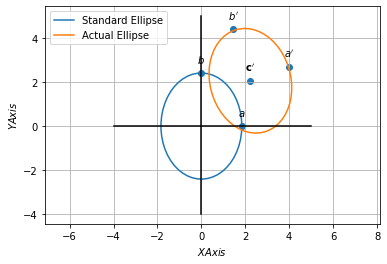
\includegraphics[width=\columnwidth]{assignment6/assignment6_fig.png}
    \caption{Graphical representation of the actual curve  $40{x^2}+36{xy}+25{y^2}-196{x}-122{y}+205=0$, which represent an ellipse.}
\label{myfig:1}
    \end{center}
\end{figure}
\end{document}
